\section{Fourier Expansions II}

\noindent
In this section we discuss Fourier expansions in terms of the
eigenfunctions of Problems~1-4 for Section~{\color{red}11.1}.

\boxit{Fourier Cosine Series}

\noindent
From  Exercise~11.1.~\hspace*{-3pt}\ref{exer:11.1.20}, the eigenfunctions
$$
1,\, \cos{\pi x\over L},
\, \cos{2\pi x\over L},\dots,
 \, \cos{n\pi x\over L},\dots
$$
 of the boundary value problem
\begin{equation} \label{eq:11.3.1}
y''+\lambda y=0,\quad y'(0)=0,\quad y'(L)=0
\end{equation}
(Problem~2)  are orthogonal on $[0,L]$.
 If $f $ is integrable on $[0,L]$ then the
Fourier expansion of $f$ in terms of these functions is called the
{\color{blue}\it Fourier cosine series of $f$ on $[0,L]$\/}. This series is
$$
a_0+\sum_{n=1}^\infty a_n\cos{n\pi x\over L},
$$
where
$$
a_0={\dst\int_0^Lf(x)\,dx\over\dst\int_0^L\,dx}={1\over
L}\int_0^Lf(x)\,dx
$$
and
$$
a_n={\dst\int_0^Lf(x)\cos{n\pi x\over L}\,dx\over\dst\int_0^L
\cos^2{n\pi x\over L}\,dx}={2\over L}\int_0^Lf(x)\cos{n\pi x\over
L}\,dx,\quad n=1,2,3,\dots.
$$
Comparing this definition with
Theorem~\ref{exer:11.2.6}\part{a} shows that the Fourier cosine
series of $f$ on $[0,L]$ is  the Fourier series of
 the  function
$$
f_1(x)=
\left\{\begin{array}{cl}
f(-x),&-L<x<0,\\f(x),&\phantom{-}0\le x\le L,
\end{array}\right.
$$
obtained by extending  $f$ over $[-L,L]$ as an even
function (Figure~\ref{figure:11.3.1}).

\begin{figure}[tbp]
  \centering\color{blue}
  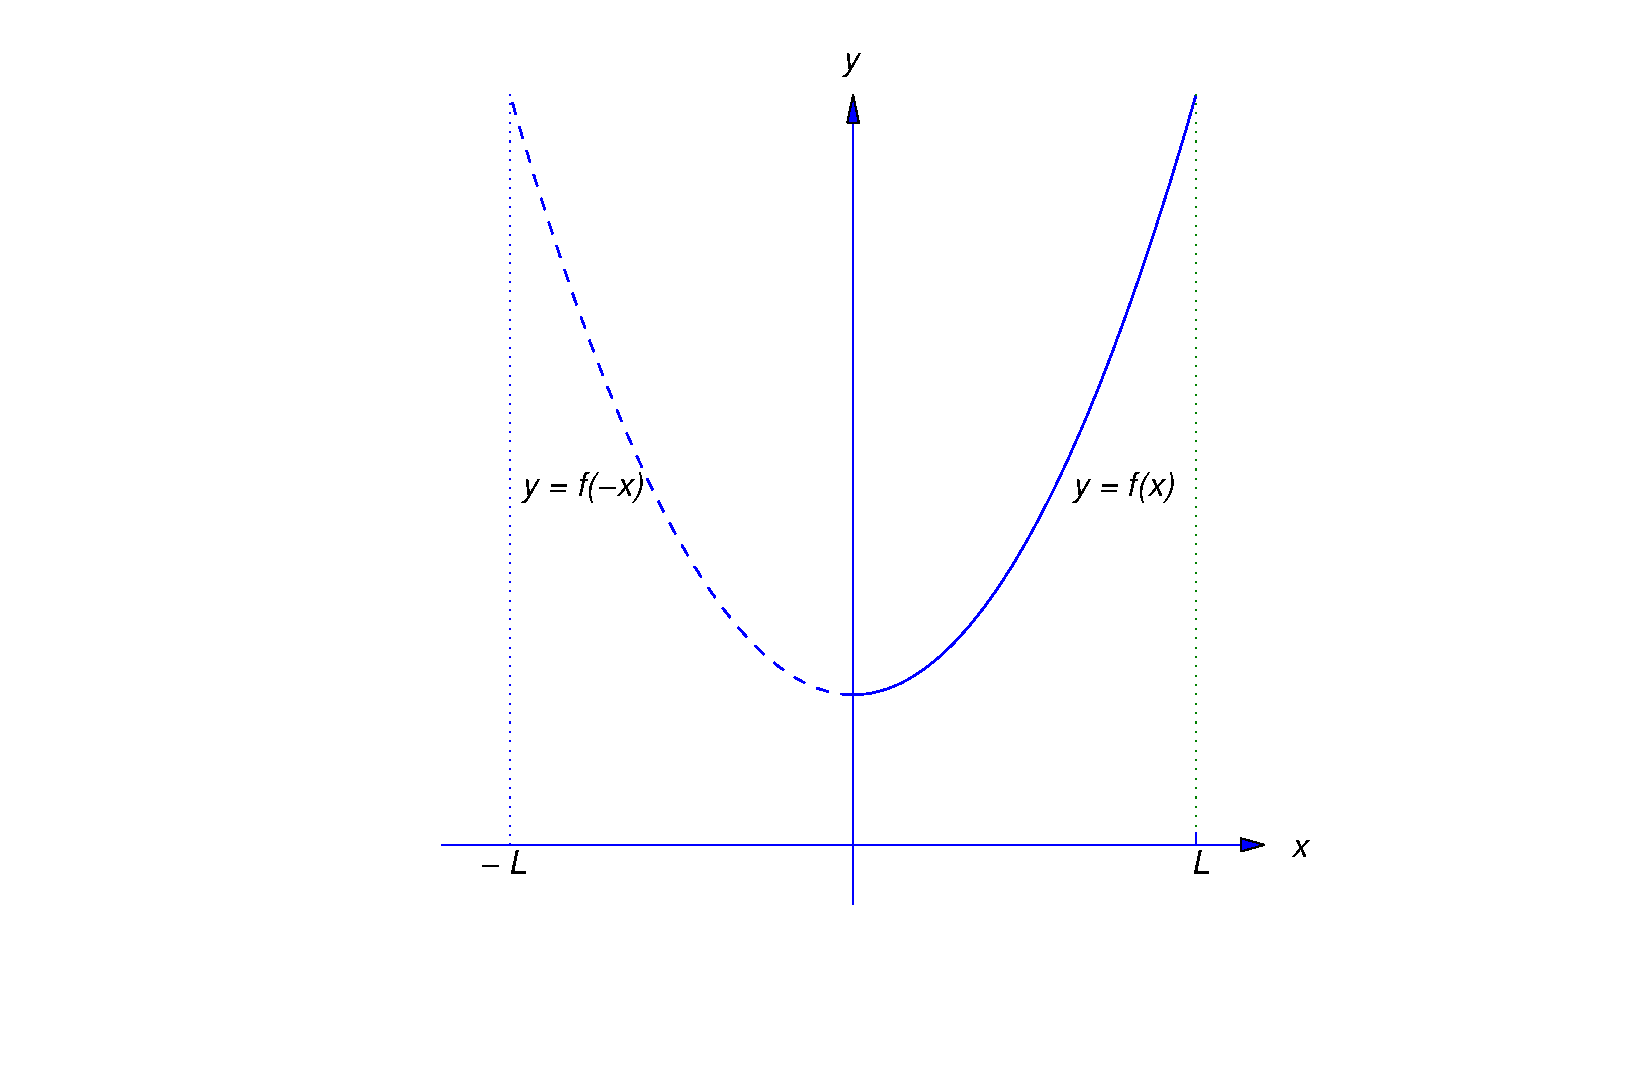
\includegraphics[bb=-78 148 689 643,width=5.67in,height=3.66in,keepaspectratio]{fig110301}
  \caption{}
  \label{figure:11.3.1}
\end{figure}

Applying
Theorem~\ref{thmtype:11.2.4} to $f_1$ yields the next
theorem.

\begin{theorem}\color{blue} \label{thmtype:11.3.1}
If $f$ is piecewise smooth on $[0,L]$, then the Fourier cosine series
$$
C(x)=a_0+\sum_{n=1}^\infty a_n\cos{n\pi x\over L}
$$
of $f$
on $[0,L]$,
with
$$
a_0={1\over L}\int_0^Lf(x)\,dx
\mbox{\quad and \quad}
a_n={2\over L}\int_0^Lf(x)\cos{n\pi x\over L}\,dx,\quad n=1,2,3,\dots,
$$
 converges for all $x$ in $[0,L]$;     moreover,
$$
C(x)=
\left\{\begin{array}{cl}
f(0+)&\mbox{if }x=0  \\
f(x)&\mbox{if $0<x<L$ and $f$ is continuous at $x  $}\\[2\jot]
\dst{f(x-)+f(x+)\over2}&\mbox{if $0<x<L$ and $f$ is discontinuous at
$x  $}\\[2\jot]
f(L-)&\mbox{if }x=L.
\end{array}\right.
$$
\end{theorem}

\begin{example}\label{example:11.3.1} \rm
Find the Fourier cosine series of $f(x)=x$ on $[0,L]$.
\end{example}

\solution
 The coefficients are
$$
a_0={1\over L}\int_0^Lx\,dx={1\over
L}{x^2\over2}
\lims0L={L\over2}
$$
and, if $n\ge1$
\begin{eqnarray*}
a_n&=&{2\over L}\int_0^Lx\cos{n\pi x\over L}\,dx
={2\over n\pi}\left[x\sin{n\pi x\over L}\lims0L-
\int_0^L
\sin{n\pi x\over L}\,dx\right]\\
&=&-{2\over n\pi}\int_0^L
\sin{n\pi x\over L}\,dx
={2L\over n^2\pi^2}\cos{n\pi x\over L}\lims0L
={2L\over
n^2\pi^2}[(-1)^n-1]\\
&=&
\left\{\begin{array}{cl}
\dst-{4L\over(2m-1)^2\pi^2}&\mbox{if  $n=2m-1$},\\
0&\mbox{if $n=2m$}.
\end{array}\right.
\end{eqnarray*}
Therefore
$$
C(x)=\dst{L\over2}-{4L\over\pi^2}\sum_{n=1}^\infty{1\over(2n-1)^2}
\cos{(2n-1)\pi x\over L}.
$$
Theorem~\ref{thmtype:11.3.1} implies that
$$
C(x)=x,\quad 0\le x\le L.
$$

\boxit{Fourier Sine Series}

\noindent
From   Exercise~11.1.~\hspace*{-3pt}\ref{exer:11.1.19},  the eigenfunctions
$$
\sin{\pi x\over L},
\, \sin{2\pi x\over L},\dots,
 \, \sin{n\pi x\over L},\dots
$$
 of the boundary value problem
$$
y''+\lambda y=0,\quad y(0)=0,\quad y(L)=0
$$
(Problem~1)  are orthogonal on $[0,L]$.
 If $f$ is integrable on $[0,L]$ then the
Fourier expansion of $f$ in terms of these functions is called the
{\color{blue}\it Fourier sine series of $f$ on $[0,L]$\/}. This series is
$$
\sum_{n=1}^\infty b_n\sin{n\pi x\over L},
$$
where
$$
b_n={\dst\int_0^Lf(x)\sin{n\pi x\over L}\,dx\over\dst\int_0^L
\sin^2{n\pi x\over L}\,dx}={2\over L}\int_0^Lf(x)\sin{n\pi x\over
L}\,dx,\quad n=1,2,3,\dots.
$$
Comparing this definition with
Theorem~\ref{exer:11.2.6}\part{b} shows that the Fourier sine
series of $f$ on $[0,L]$ is the Fourier series of
 the  function
$$
f_2(x)=
\left\{\begin{array}{cl}
-f(-x),&-L<x<0,\\f(x),&\phantom{-}0\le x\le L,
\end{array}\right.
$$
obtained by extending  $f$ over $[-L,L]$ as an odd
function  (Figure~\ref{figure:11.3.2}).

\begin{figure}[tbp]
  \centering\color{blue}
  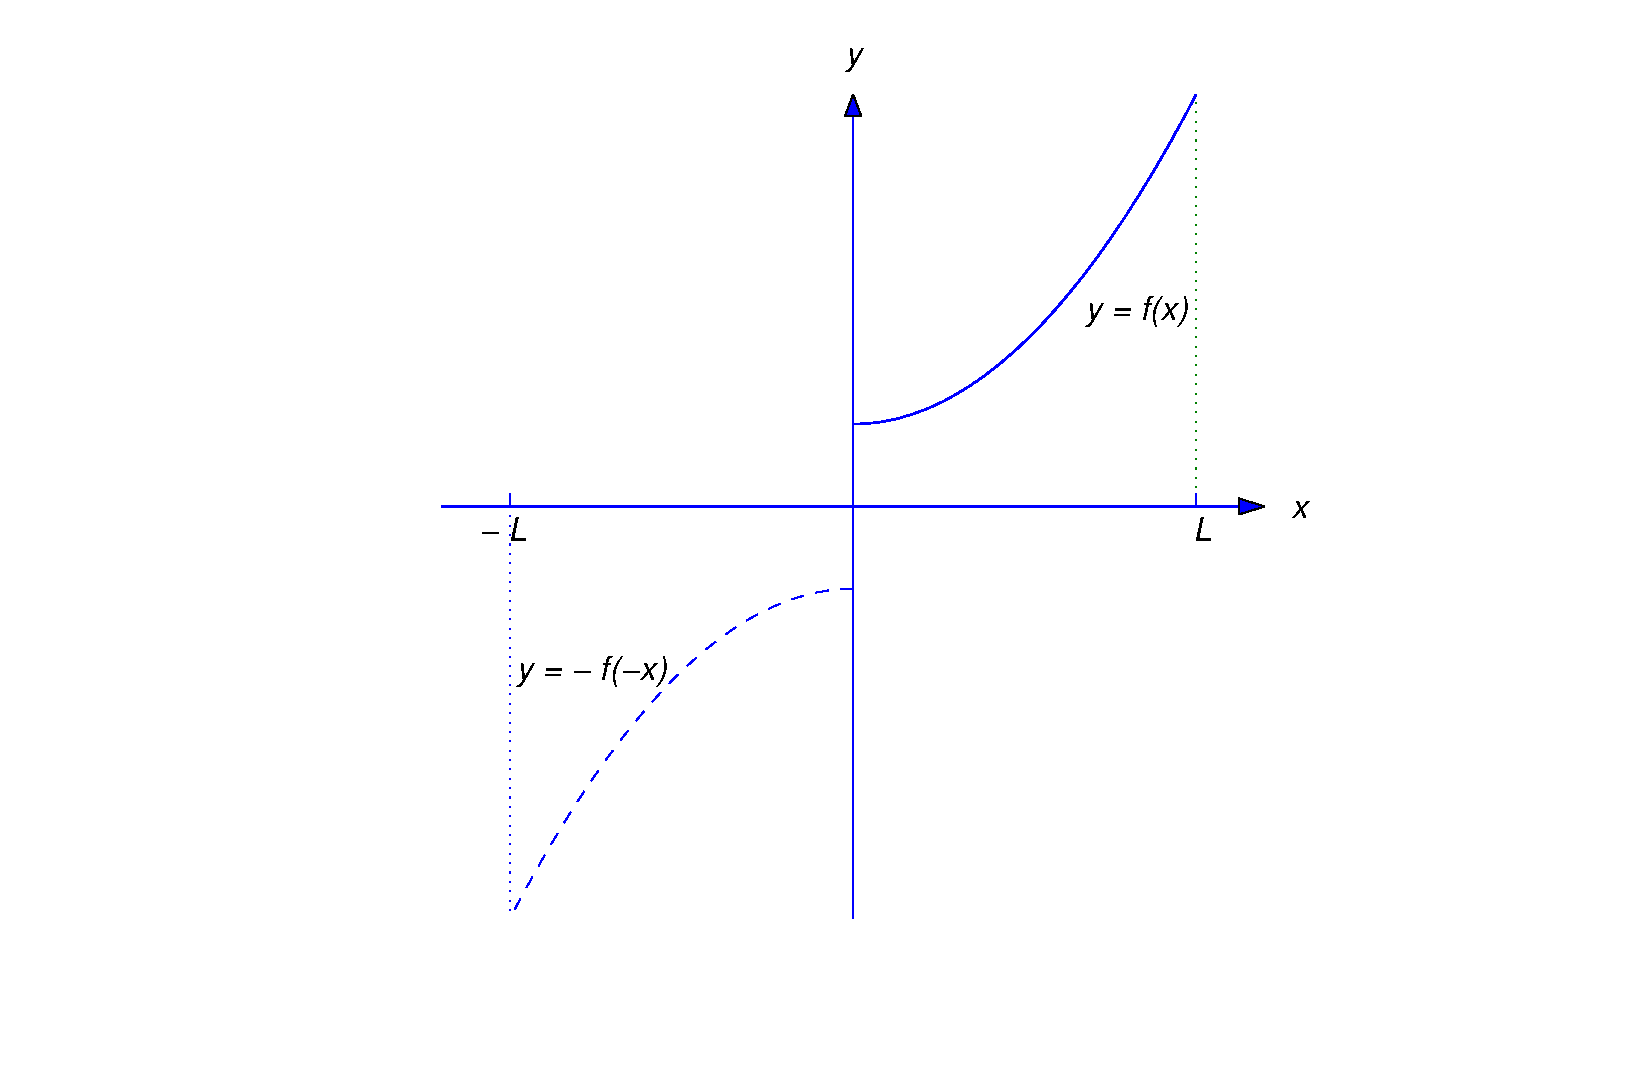
\includegraphics[bb=-78 148 689 643,width=5.67in,height=3.66in,keepaspectratio]{fig110302}
  \caption{}
  \label{figure:11.3.2}
\end{figure}

Applying
Theorem~11.2.4 to $f_2$ yields the next
theorem.

\begin{theorem}\color{blue} \label{thmtype:11.3.2}
If $f$ is piecewise smooth on $[0,L]$, then the Fourier sine series
$$
S(x)=\sum_{n=1}^\infty b_n\sin{n\pi x\over L}
$$
of $f$
on $[0,L]$,
with
$$
b_n={2\over L}\int_0^Lf(x)\sin{n\pi x\over L}\,dx,
$$
 converges for all $x$ in $[0,L]$; moreover,
$$
S(x)=
\left\{\begin{array}{cl}
0&\mbox{if }x=0  \\
f(x)&\mbox{if $0<x<L$ and $f$ is continuous at $x  $}\\[2\jot]
\dst{f(x-)+f(x+)\over2}&\mbox{if $0<x<L$ and $f$ is discontinuous at
$x  $}\\[2\jot]
0&\mbox{if }x=L.
\end{array}\right.
$$
\end{theorem}

\begin{example}\label{example:11.3.2} \rm
Find the Fourier sine series of $f(x)=x$ on $[0,L]$.
\end{example}

\solution
 The coefficients are
\begin{eqnarray*}
b_n&=&{2\over L}\int_0^Lx\sin{n\pi x\over L}\,dx
=-{2\over n\pi}\left[x\cos{n\pi x\over L}\lims0L-
\int_0^L
\cos{n\pi x\over L}\,dx\right]\\
&=& (-1)^{n+1}{2L\over n\pi}+{2L\over n^2\pi^2}\sin{n\pi x\over
L}\lims0L =(-1)^{n+1}{2L\over n\pi}.
\end{eqnarray*}
Therefore
$$
S(x)=\dst-{2L\over\pi}\sum_{n=1}^\infty{(-1)^n\over n}
\sin{n\pi x\over L}.
$$
Theorem~\ref{thmtype:11.3.2} implies that
$$
S(x)=
\left\{\begin{array}{cl}
x,&0\le x< L,\\0,& x=L.
\end{array}\right.
$$

\boxit{Mixed Fourier Cosine Series}

\noindent
From Exercise~11.1.~\hspace*{-3pt}\ref{exer:11.1.22}, the eigenfunctions
$$
 \cos{\pi x\over 2L},
\, \cos{3\pi x\over 2L},\dots,
 \, \cos{(2n-1)\pi x\over 2L},\dots
$$
 of the boundary value problem
\begin{equation} \label{eq:11.3.2}
y''+\lambda y=0,\quad y'(0)=0,\quad y(L)=0
\end{equation}
(Problem~4) are orthogonal on $[0,L]$.
 If $f$ is integrable on $[0,L]$ then the
Fourier expansion of $f$ in terms of these functions  is
$$
\sum_{n=1}^\infty c_n\cos{(2n-1)\pi x\over2L},
$$
where
$$
c_n={\dst\int_0^Lf(x)\cos{(2n-1)\pi x\over2L}\,dx\over\dst\int_0^L
\cos^2{(2n-1)\pi x\over L}\,dx}={2\over L}\int_0^Lf(x)\cos{(2n-1)\pi
x\over2L}\,dx.
$$

We'll  call this expansion the  {\color{blue}\it mixed Fourier cosine
series\/} of $f$ on $[0,L]$, because the boundary conditions
of (\ref{eq:11.3.2}) are ``mixed'' in that they require $y$
to be zero at
 one boundary point and $y'$ to be  zero at the other. By contrast,
the ``ordinary'' Fourier cosine series is associated with
(\ref{eq:11.3.1}), where the boundary conditions require that $y'$
be zero at both endpoints.

It can be shown (Exercise~\ref{exer:11.3.57}) that
 the mixed Fourier cosine series
of $f$ on $[0,L]$
is simply the restriction to  $[0,L]$ of the Fourier
cosine series  of
$$
f_3(x)=
\left\{\begin{array}{cl}
f(x),&0\le x\le L,\\-f(2L-x),&L< x\le 2L
\end{array}\right.
$$
on $[0,2L]$ (Figure~\ref{figure:11.3.3}).

\begin{figure}[H]
  \centering\color{blue}
  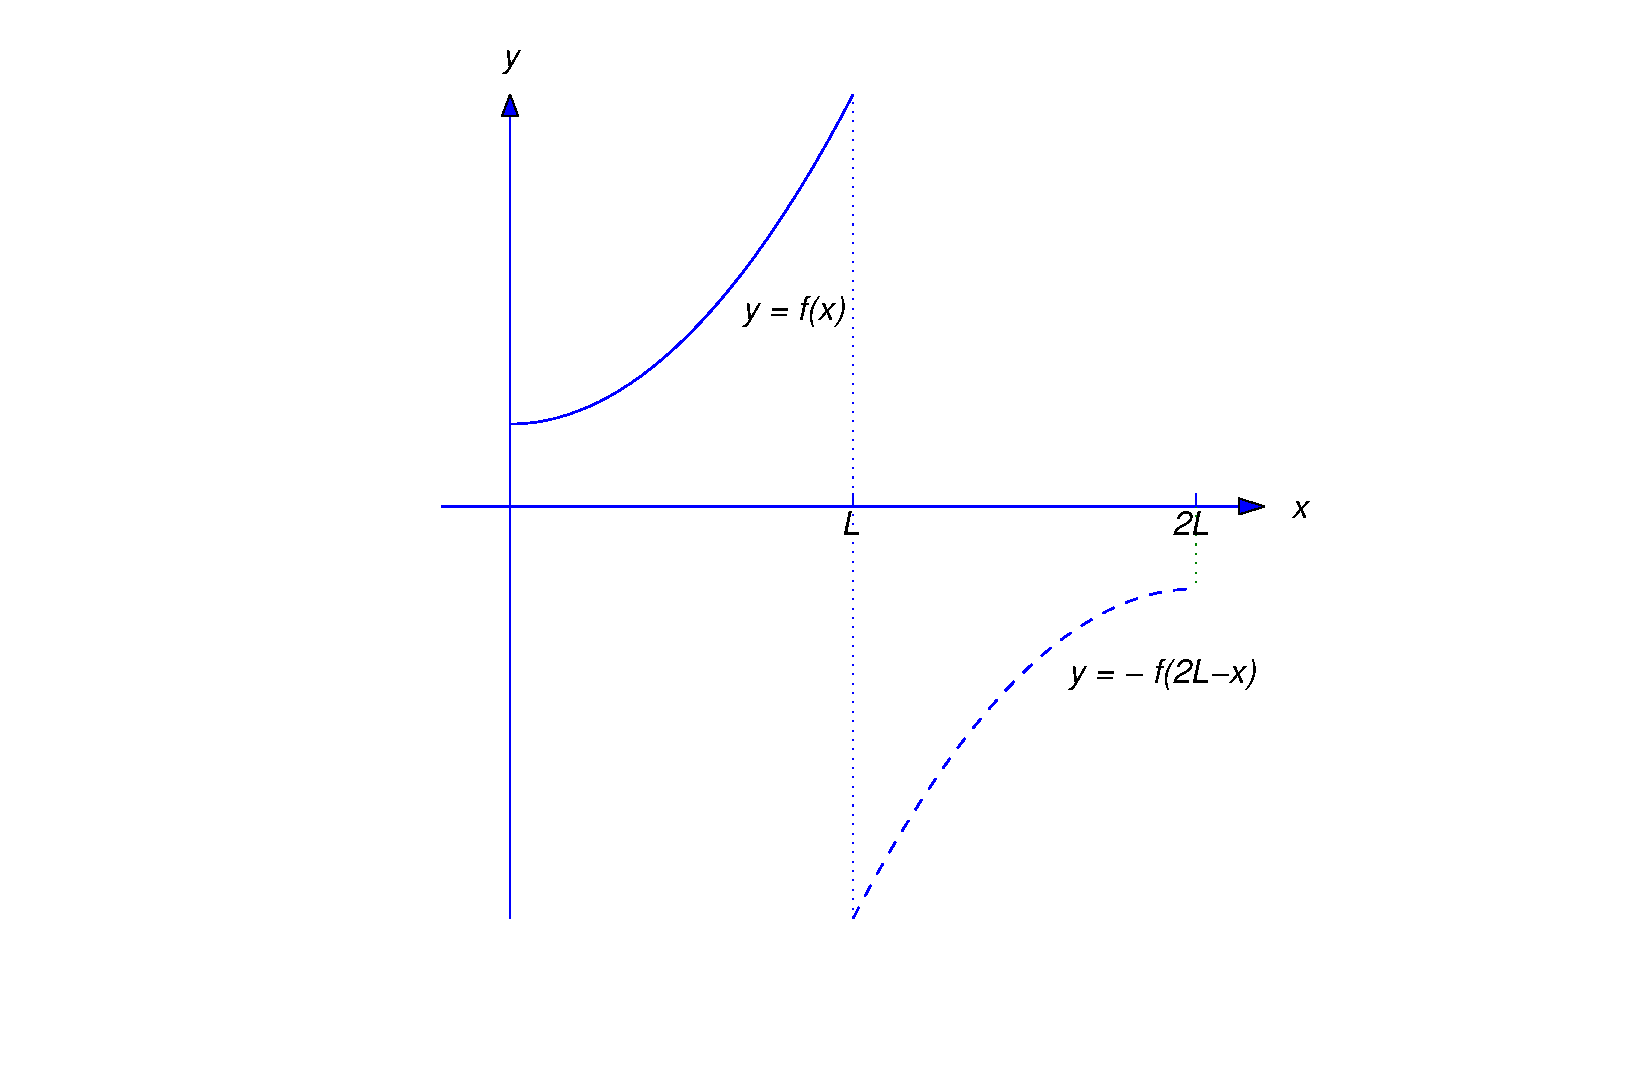
\includegraphics[bb=-78 148 689 643,width=5.67in,height=3.66in,keepaspectratio]{fig110303}
  \caption{}
  \label{figure:11.3.3}
\end{figure}

Applying  Theorem~\ref{thmtype:11.3.1}  with $f$ replaced by $f_3$ and $L$
replaced by $2L$ yields the next theorem.

\begin{theorem}\color{blue} \label{thmtype:11.3.3}
If  $f$ is piecewise smooth on $[0,L]$, then
the mixed Fourier cosine series
$$
C_M(x)=\sum_{n=1}^\infty c_n\cos{(2n-1)\pi x\over2L}
$$
of $f$ on $[0,L]$,
with
$$
c_n={2\over L}\int_0^Lf(x)\cos{(2n-1)\pi x\over2L}\,dx,
$$
 converges for all $x$ in $[0,L]$; moreover,
$$
C_M(x)=
\left\{\begin{array}{cl}
f(0+)&\mbox{if $x=0$}  \\
f(x)&\mbox{if $0<x<L$ and $f$ is continuous at $x$  }\\[2\jot]
\dst{f(x-)+f(x+)\over2}&\mbox{if $0<x<L$ and $f$ is discontinuous at
$x$  }\\[2\jot]
0&\mbox{if $x=L$.}
\end{array}\right.
$$
\end{theorem}

\begin{example}\label{example:11.3.3} \rm
Find  the mixed Fourier cosine series of
$f(x)=x-L$ on $[0,L]$.
\end{example}

\solution
 The coefficients are
\begin{eqnarray*}
c_n&=&{2\over L}\int_0^L(x-L)\cos{(2n-1)\pi x\over2L}\,dx\\
&=&{4\over(2n-1)\pi}\left[(x-L)\sin{(2n-1)\pi
x\over2L}\lims0L-\int_0^L
\sin{(2n-1)\pi x\over2L}\,dx\right]\\
&=&{8L\over(2n-1)^2\pi^2}
\cos{(2n-1)\pi x\over2L}\lims0L
=-{8L\over(2n-1)^2\pi^2}.
\end{eqnarray*}
Therefore
$$
C_M(x)=-{8L\over\pi^2}\sum_{n=1}^\infty{1\over(2n-1)^2}
\cos{(2n-1)\pi x\over2L}.
$$
Theorem~\ref{thmtype:11.3.3} implies that
$$
C_M(x)= x-L,\quad 0\le x\le L.
$$

\boxit{Mixed Fourier Sine Series}

\noindent
From  Exercise~11.1.~\hspace*{-3pt}\ref{exer:11.1.21},  the eigenfunctions
$$
 \sin{\pi x\over 2L},
\, \sin{3\pi x\over 2L},\dots,
 \, \sin{(2n-1)\pi x\over 2L},\dots
$$
of the boundary value problem
$$
y''+\lambda y=0,\quad y(0)=0,\quad y'(L)=0
$$
(Problem~3)   are orthogonal on $[0,L]$.
 If $f$ is integrable on $[0,L]$, then the
Fourier expansion of $f$ in terms of these functions
is
$$
\sum_{n=1}^\infty d_n\sin{(2n-1)\pi x\over2L},
$$
where
$$
d_n={\dst\int_0^Lf(x)\sin{(2n-1)\pi x\over2L}\,dx\over\dst\int_0^L
\sin^2{(2n-1)\pi x\over2L}\,dx}={2\over L}\int_0^Lf(x)\sin{(2n-1)\pi
x\over2L}\,dx.
$$
We'll  call this expansion the  {\color{blue}\it mixed Fourier sine
series\/} of $f$ on $[0,L]$.

It can be shown (Exercise~\ref{exer:11.3.58}) that
 the mixed Fourier sine series
of $f$ on $[0,L]$
is simply the restriction to  $[0,L]$ of the Fourier
sine series of
$$
f_4(x)=
\left\{\begin{array}{cl}
f(x),&0\le x\le L,\\f(2L-x),&L< x\le 2L,
\end{array}\right.
$$
on $[0,2L]$ (Figure~\ref{figure:11.3.4}).

\begin{figure}[H]
  \centering\color{blue}
  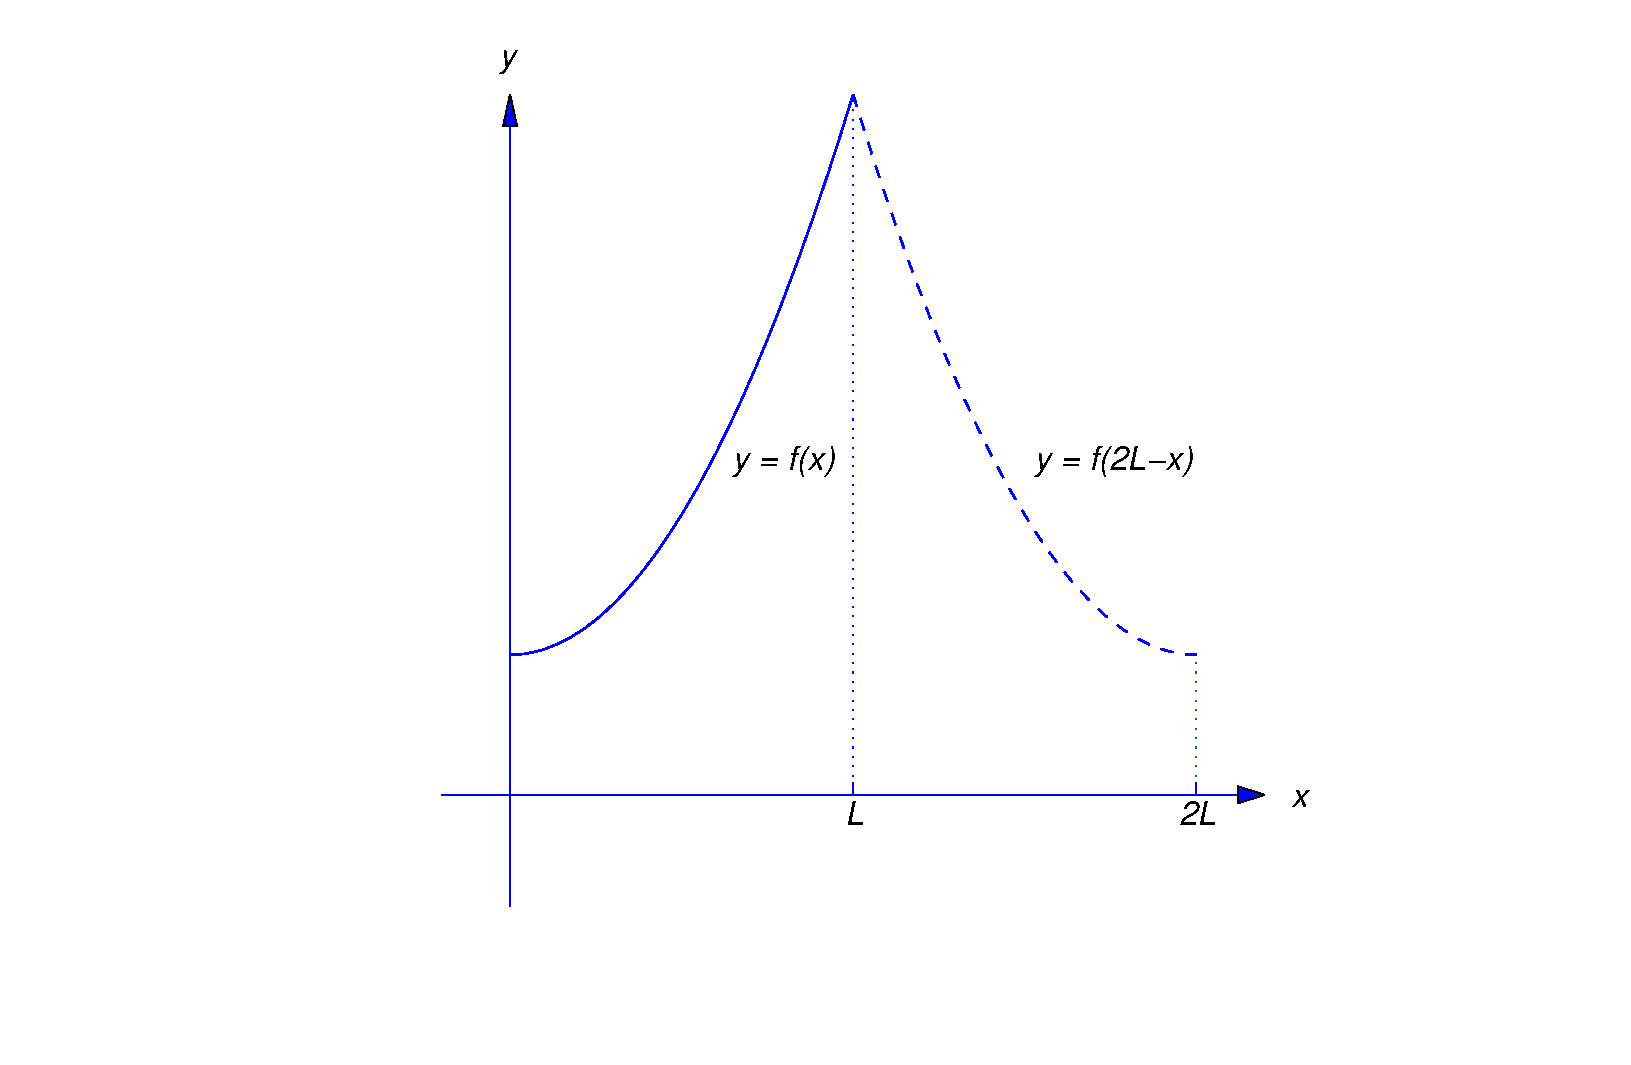
\includegraphics[bb=-78 148 689 643,width=5.67in,height=3.66in,keepaspectratio]{fig110304}
  \caption{}
  \label{figure:11.3.4}
\end{figure}

Applying Theorem~\ref{thmtype:11.3.2} with $f$ replaced by $f_4$ and $L$
replaced by $2L$ yields the next theorem.

\begin{theorem}\color{blue} \label{thmtype:11.3.4}
If $f$ is piecewise smooth on $[0,L]$, then the mixed Fourier
sine series
$$
S_M(x)=\sum_{n=1}^\infty d_n\sin{(2n-1)\pi x\over2L}
$$
of $f$ on $[0,L]$, with
$$
d_n={2\over L}\int_0^Lf(x)\sin{(2n-1)\pi x\over2L}\,dx,
$$
 converges for all $x$ in $[0,L]$; moreover,
$$
S_M(x)=
\left\{\begin{array}{cl}
0&\mbox{if $x=0$}  \\
f(x)&\mbox{if $0<x<L$ and $f$ is continuous at $x$  }\\[2\jot]
\dst{f(x-)+f(x+)\over2}&\mbox{if $0<x<L$ and $f$ is discontinuous at
$x$  }\\[2\jot]
f(L-)&\mbox{if $x=L$.}
\end{array}\right.
$$
\end{theorem}

\begin{example}\label{example:11.3.4} \rm
Find the mixed Fourier sine series of $f(x)=x$ on $[0,L]$.
\end{example}

\solution
 The coefficients are
\begin{eqnarray*}
d_n&=&{2\over L}\int_0^Lx\sin{(2n-1)\pi x\over2L}\,dx\\
&=&-{4\over(2n-1)\pi}\left[x\cos{(2n-1)\pi
x\over2L}\lims0L-
\int_0^L
\cos{(2n-1)\pi x\over2L}\,dx\right]\\
&=&{4\over(2n-1)\pi}
\int_0^L
\cos{(2n-1)\pi x\over2L}\,dx\\
&=&{8L\over(2n-1)^2\pi^2}\sin{(2n-1)\pi
x\over2L}\lims0L=(-1)^{n+1}{8L\over(2n-1)^2\pi^2}.
\end{eqnarray*}
Therefore
$$
S_M(x)=-{8L\over\pi^2}\sum_{n=1}^\infty{(-1)^n\over(2n-1)^2}
\sin{(2n-1)\pi x\over2L}.
$$
Theorem~\ref{thmtype:11.3.4} implies that
$$
S_M(x)=x,\quad 0\le x\le L.
$$

\boxit{A Useful Observation}

\noindent
In applications involving expansions in
terms of the eigenfunctions of Problems~1-4, the functions being
expanded
 are often  polynomials that  satisfy the boundary conditions
of the problem under consideration. In this case the next theorem
presents an
 efficient way  to obtain the
coefficients in the expansion.

\begin{theorem}\color{blue}  \label{thmtype:11.3.5}
\mbox{}\\

\part{a}
If $f'(0)=f'(L)=0$, $f''$ is continuous, and $f'''$ is piecewise
continuous  on $[0,L]$, then
\begin{equation} \label{eq:11.3.3}
f(x)=a_0+\sum_{n=1}^\infty a_n\cos{n\pi x\over L},
\quad 0\le x\le L,
\end{equation}
with
\begin{equation} \label{eq:11.3.4}
a_0={1\over L}\int_0^L f(x)\,dx \mbox{\quad and \quad}
a_n= {2L^2\over n^3\pi^3}\int_0^L f'''(x)\sin{n\pi
x\over L}\,dx,
\quad n\ge1.
\end{equation}

Now suppose $f'$ is continuous and $f''$ is piecewise
continuous on $[0,L]$.

\part{b}
If  $f(0)=f(L)=0$, then
$$
f(x)=\sum_{n=1}^\infty b_n\sin{n\pi x\over L},
\quad 0\le x\le L,
$$
with
\begin{equation} \label{eq:11.3.5}
b_n=-{2L\over n^2\pi^2}\int_0^L f''(x)\sin{n\pi
x\over L}\,dx.
\end{equation}

\part{c}
If  $f'(0)=f(L)=0$, then
$$
f(x)=
\sum_{n=1}^\infty c_n\cos{(2n-1)\pi x\over2L},
\quad 0\le x\le L,
$$
with
\begin{equation} \label{eq:11.3.6}
c_n=-{8L\over(2n-1)^2\pi^2}\int_0^L f''(x)\cos{(2n-1)\pi x\over2L}
\,dx.
\end{equation}

\part{d}
If  $f(0)=f'(L)=0$, then
$$
f(x)=
\sum_{n=1}^\infty d_n\sin{(2n-1)\pi x\over2L},
\quad 0\le x\le L,
$$
with
\begin{equation} \label{eq:11.3.7}
d_n=-{8L\over(2n-1)^2\pi^2}\int_0^L f''(x)\sin{(2n-1)\pi x\over2L}
\,dx.
\end{equation}
\end{theorem}

\proof  We'll prove \part{a} and leave the rest to you
(Exercises~\ref{exer:11.3.35}, \ref{exer:11.3.42}, and \ref{exer:11.3.50}).  Since
$f$ is continuous on
$[0,L]$, Theorem~\ref{thmtype:11.3.1} implies (\ref{eq:11.3.3}) with $a_0$,
$a_1$, $a_2$,... as defined in Theorem~\ref{thmtype:11.3.1}. We already
know that
$a_0$ is as in
(\ref{eq:11.3.4}). If  $n\ge1$, integrating twice by parts yields
\begin{eqnarray*}
a_n&=& {2\over L}\int_0^L f(x)\cos{n\pi x\over L}\,dx\\
&=&{2\over n\pi}\left[f(x)\sin{n\pi x\over L}\lims0L
-\int_0^Lf'(x)\sin{n\pi x\over L}\,dx\right]\\
&=&-{2\over n\pi}
\int_0^Lf'(x)\sin{n\pi x\over L}\,dx
\mbox{ (since $\sin0=\sin n\pi=0$)}\\
&=&{2L\over n^2\pi^2}\left[f'(x)\cos{n\pi x\over L}\lims0L
-\int_0^Lf''(x)\cos{n\pi x\over L}\right]\,dx\\
&=&
-{2L\over n^2\pi^2}\int_0^Lf''(x)\cos{n\pi x\over L}\,dx
\mbox{ (since $f'(0)=f'(L)=0$)}\\
&=&-{2L^2\over n^3\pi^3}\left[f''(x)\sin{n\pi x\over L}\lims0L
-\int_0^Lf'''(x)\sin{n\pi x\over L}\,dx\right]\\
&=&
{2L^2\over n^3\pi^3}\int_0^Lf'''(x)\sin{n\pi x\over L}\,dx
\mbox{ (since $\sin0=\sin n\pi=0$).}
\end{eqnarray*}
(By an argument similar to one used in the proof of Theorem~8.3.1,
 the last integration by parts is legitimate
in the case where $f'''$ is undefined at finitely many points in
$[0,L]$, so long as it's piecewise continuous on $[0,L]$.)
This completes the proof.

\begin{example}\label{example:11.3.5} \rm
Find the Fourier cosine expansion of $f(x)=x^2(3L-2x)$
on $[0,L]$.
\end{example}

\solution
Here
$$
a_0={1\over L}\int_0^L(3Lx^2-2x^3)\,dx={1\over
L}\left(Lx^3-{x^4\over2}
\right)\lims0L={L^3\over2}
$$
and
$$
a_n={2\over L}\int_0^L(3Lx^2-2x^3)\cos{n\pi x\over L}\,dx,\quad n\ge1.
$$
Evaluating this integral directly is laborious.
However, since $f'(x)=6Lx-6x^2$, we see that $f'(0)=f'(L)=0$.
Since $f'''(x)=-12$, we see from (\ref{eq:11.3.4}) that if $n\ge1$ then
\begin{eqnarray*}
a_n&=&-{24L^2\over n^3\pi^3}\int_0^L\sin{n\pi x\over L}\,dx
={24L^3\over n^4\pi^4}\cos{n\pi x\over L}\lims0L={24L^3\over
n^4\pi^4}[(-1)^n-1]\\
&=&
\left\{\begin{array}{cl}
\dst-{48L^3\over(2m-1)^4\pi^4}&\mbox{if  $n=2m-1$},\\
0&\mbox{if $n=2m$.}
\end{array}\right.
\end{eqnarray*}
Therefore
$$
C(x)={L^3\over2}-{48L^3\over\pi^4}\sum_{n=1}^\infty{1\over
(2n-1)^4}\cos{(2n-1)\pi x\over L}.
$$

\begin{example}\label{example:11.3.6} \rm
Find the Fourier sine expansion of
$f(x)=x(x^2-3Lx+2L^2)$
on $[0,L]$.
\end{example}

\solution
Since $f(0)=f(L)=0$ and $f''(x)=6(x-L)$, we see from (\ref{eq:11.3.5})
that
\begin{eqnarray*}
b_n&=&-
{12L\over n^2\pi^2}\int_0^L(x-L)\sin{n\pi x\over L}\,dx\\
&=&{12L^2\over n^3\pi^3}\left[(x-L)\cos{n\pi x\over L}\lims0L
-\int_0^L\cos{n\pi x\over L}\,dx\right]\\
&=&{12L^2\over n^3\pi^3}\left[L-\frac{L}{n\pi}\sin\frac{n\pi
x}{L}\lims0L\right]
={12L^3\over
n^3\pi^3}.
\end{eqnarray*}
Therefore
$$
S(x)=\dst{12L^3\over\pi^3}\sum_{n=1}^\infty{1\over n^3}
\sin{n\pi x\over L}.
$$

\begin{example}\label{example:11.3.7} \rm
Find  the mixed Fourier cosine expansion of
$f(x)=3x^3-4Lx^2+L^3$
on $[0,L]$.
\end{example}

\solution
Since $f'(0)=f(L)=0$ and $f''(x)=2(9x-4L)$, we see from (\ref{eq:11.3.6})
that
\begin{eqnarray*}
c_n&=&
-{16L\over(2n-1)^2\pi^2}
\int_0^L(9x-4L)\cos{(2n-1)\pi x\over2L}\,dx\\
&=&-{32L^2\over(2n-1)^3\pi^3}\left[(9x-4L)\sin{(2n-1)\pi x\over2L}
\lims0L-9\int_0^L\sin{(2n-1)\pi x\over2L}\right]\,dx\\
&=&-{32L^2\over(2n-1)^3\pi^3}
\left[(-1)^{n+1}5L+{18L\over(2n-1)\pi}\cos{(2n-1)\pi x\over2L}
\lims0L\right] \\
&=&{32L^3\over(2n-1)^3\pi^3}
\left[(-1)^n5+{18\over(2n-1)\pi}\right].
\end{eqnarray*}
Therefore
$$
C_M(x)=\dst{32L^3\over\pi^3}\sum_{n=1}^\infty{1\over(2n-1)^3}\left[
(-1)^n5+{18\over(2n-1)\pi}\right]\cos{(2n-1)\pi
x\over2L}.
$$

\begin{example}\label{example:11.3.8} \rm
Find  the mixed Fourier  sine expansion of
$$
f(x)=x(2x^2-9Lx+12L^2)
$$
on $[0,L]$.
\end{example}

\solution
Since $f(0)=f'(L)=0$, and $f''(x)=6(2x-3L)$, we see from (\ref{eq:11.3.7})
that
\begin{eqnarray*}
d_n&=&-\dst{48L\over(2n-1)^2\pi^2}\int_0^L(2x-3L)
\sin{(2n-1)\pi x\over2L}\,dx\\
&=&\dst{96L^2\over(2n-1)^3\pi^3}\left[(2x-3L)\cos{(2n-1)\pi
x\over2L}\lims0L-2\int_0^L\cos{(2n-1)\pi x\over2L}\,dx\right]\\
&=&\dst{96L^2\over(2n-1)^3\pi^3}\left[3L-{4L\over(2n-1)\pi}
\sin{(2n-1)\pi x\over2L}\lims0L\right]\\
&=&\dst{96L^3\over(2n-1)^3\pi^3}\left[3+(-1)^n{4\over(2n-1)\pi}\right].
\end{eqnarray*}
Therefore
$$
S_M(x)
=\dst{96L^3\over\pi^3}\sum_{n=1}^\infty
{1\over(2n-1)^3}\left[3+(-1)^n{4\over(2n-1)\pi}\right]\sin{(2n-1)\pi
x\over2L}.
$$

\exercises
\noindent
In exercises marked by \Cex\, graph $f$
and some partial sums of the required series. If the interval
is $[0,L]$, choose a specific value of $L$ for the graph.

\noindent
\emph{In Exercises~\ref{exer:11.3.1}-\ref{exer:11.3.10} find the Fourier
cosine series.}

\begin{exerciselist}

\item\label{exer:11.3.1}
$f(x)=x^2$;  \quad $[0,L]$

\item\label{exer:11.3.2}
\Cex $f(x)=1-x$;   \quad $[0,1]$

\item\label{exer:11.3.3} \Cex
$f(x)=x^2-2Lx$;   \quad $[0,L]$

\item\label{exer:11.3.4}
$f(x)=\sin kx$\, ($k\ne$ integer);\quad    $[0,\pi]$

\item\label{exer:11.3.5} \Cex
$f(x)=
\left\{\begin{array}{cl}
1,&0\le x\le{L\over2}\\0,&{L\over2}<x<L;
\end{array}\right.$ \quad $[0,L]$

\item\label{exer:11.3.6}
$f(x)=x^2-L^2$;   \quad $[0,L]$

\item\label{exer:11.3.7}
 $f(x)=(x-1)^2$;  \quad $[0,1]$

\item\label{exer:11.3.8}
$f(x)=e^x$;   \quad $[0,\pi]$

\item\label{exer:11.3.9} \Cex
$f(x)=x(L-x)$;  \quad $[0,L]$

\item\label{exer:11.3.10} \Cex
$f(x)=x(x-2L)$;  \quad $[0,L]$

\exercisetext{
In Exercises~\ref{exer:11.3.11}-\ref{exer:11.3.17} find the Fourier sine
series.}

\item\label{exer:11.3.11}  \Cex
$f(x)=1$;  \quad$[0,L]$

\item\label{exer:11.3.12}
\Cex $f(x)=1-x$;   \quad $[0,1]$

\item\label{exer:11.3.13}
$f(x)=\cos kx$\, ($k\ne$ integer);  \quad $[0,\pi]$

\item\label{exer:11.3.14} \Cex
$f(x)=
\left\{\begin{array}{cl}
1,&0\le x\le{L\over2}\\0,&{L\over2}<x<L;
\end{array}\right.$ \quad $[0,L]$

\item\label{exer:11.3.15} \Cex
$f(x)=
\left\{\begin{array}{cl}
x,&0\le x\le{L\over2},\\L-x,&{L\over2}\le x\le L;
\end{array}\right.$
\quad $[0,L]$.

\item\label{exer:11.3.16} \Cex
$f(x)=x\sin x$;   \quad $[0,\pi]$

\item\label{exer:11.3.17}
$f(x)=e^x$;   \quad $[0,\pi]$

\exercisetext{
In Exercises~\ref{exer:11.3.18}-\ref{exer:11.3.24} find the mixed Fourier
cosine series.}

\item\label{exer:11.3.18}  \Cex
$f(x)=1$;  \quad$[0,L]$

\item\label{exer:11.3.19}
$f(x)=x^2$;  \quad $[0,L]$

\item\label{exer:11.3.20}
\Cex $f(x)=x$;   \quad $[0,1]$

\item\label{exer:11.3.21} \Cex
$f(x)=
\left\{\begin{array}{cl}
1,&0\le x\le{L\over2}\\0,&{L\over2}<x<L;
\end{array}\right.$ \quad $[0,L]$

\item\label{exer:11.3.22}
$f(x)=\cos x$;   \quad $[0,\pi]$

\item\label{exer:11.3.23}
$f(x)=\sin x$;   \quad $[0,\pi]$

\item\label{exer:11.3.24} \Cex
$f(x)=x(L-x)$;  \quad $[0,L]$

\exercisetext{
In Exercises~\ref{exer:11.3.25}-\ref{exer:11.3.30} find the mixed Fourier sine
series.}

\item\label{exer:11.3.25}  \Cex
$f(x)=1$;  \quad$[0,L]$

\item\label{exer:11.3.26}
$f(x)=x^2$;  \quad $[0,L]$

\item\label{exer:11.3.27} \Cex
$f(x)=
\left\{\begin{array}{cl}
1,&0\le x\le{L\over2}\\0,&{L\over2}<x<L;
\end{array}\right.$\quad  $[0,L]$

\item\label{exer:11.3.28}
$f(x)=\cos x$;   \quad $[0,\pi]$

\item\label{exer:11.3.29}
$f(x)=\sin x$;   \quad $[0,\pi]$

\item\label{exer:11.3.30} \Cex
$f(x)=x(L-x)$;  \quad $[0,L]$.

\exercisetext{In Exercises~\ref{exer:11.3.31}-\ref{exer:11.3.34}
use Theorem~\ref{thmtype:11.3.5}\part{a} to find the  Fourier
cosine series of $f$ on~$[0,L]$.}

\item\label{exer:11.3.31}
$f(x)=3x^2(x^2-2L^2)$

\item\label{exer:11.3.32}
$f(x)=x^3(3x-4L)$

\item\label{exer:11.3.33}
$f(x)=x^2(3x^2-8Lx+6L^2)$

\item\label{exer:11.3.34}
$f(x)=x^2(x-L)^2$

\item\label{exer:11.3.35}
\begin{alist}
\item % (a)
Prove Theorem~\ref{thmtype:11.3.5}\part{b}.
\item % (b)
In addition to the assumptions of Theorem~\ref{thmtype:11.3.5}\part{b},
suppose  $f''(0)=f''(L)=0$, $f'''$ is continuous,  and $f^{(4)}$
is piecewise continuous on $[0,L]$.
Show that
$$
b_n={2L^3\over n^4\pi^4}\int_0^L f^{(4)}(x)\sin{n\pi
x\over L}\,dx,
\quad n\ge1.
$$
\end{alist}

\exercisetext{
In Exercises~\ref{exer:11.3.36}-\ref{exer:11.3.41}
use Theorem~\ref{thmtype:11.3.5}\part{b}
or, where applicable,
Exercise~$11.1$.~\hspace*{-3pt}\ref{exer:11.3.35}\part{b},
to find the Fourier sine series of $f$  on $[0,L]$.}

\item\label{exer:11.3.36}
\Cex $f(x)=x(L-x)$

\item\label{exer:11.3.37}
\Cex\quad$f(x)=x^2(L-x)$

\item\label{exer:11.3.38}
$f(x)=x(L^2-x^2)$

\item\label{exer:11.3.39}
$f(x)=x(x^3-2Lx^2+L^3)$

\item\label{exer:11.3.40}
$f(x)=x(3x^4-10L^2x^2+7L^4)$

\item\label{exer:11.3.41}
$f(x)=x(3x^4-5Lx^3+2L^4)$

\item\label{exer:11.3.42}
\begin{alist}
\item % (a)
Prove Theorem~\ref{thmtype:11.3.5}\part{c}.
\item % (b)
In addition to the assumptions of Theorem~\ref{thmtype:11.3.5}\part{c},
suppose
$f''(L)=0$, $f''$ is continuous, and $f'''$ is piecewise continuous on
$[0,L]$. Show that
$$
c_n={16L^2\over(2n-1)^3\pi^3}\int_0^L f'''(x)\sin{(2n-1)\pi x\over2L}
\,dx,\quad n\ge1.
$$
\end{alist}

\exercisetext{
In Exercises~\ref{exer:11.3.43}-\ref{exer:11.3.49}
use Theorem~\ref{thmtype:11.3.5}\part{c}
or, where applicable,
Exercise~$11.1$.~\hspace*{-3pt}\ref{exer:11.3.42}\part{b},
to find the mixed Fourier
cosine series of $f$ on $[0,L]$.}

\item\label{exer:11.3.43}
\Cex $f(x)=x^2(L-x)$

\item\label{exer:11.3.44}
$f(x)=L^2-x^2$

\item\label{exer:11.3.45}
$f(x)=L^3-x^3$

\item\label{exer:11.3.46}
$f(x)=2x^3+3Lx^2-5L^3$

\item\label{exer:11.3.47}
$f(x)=4x^3+3Lx^2-7L^3$

\item\label{exer:11.3.48}
$f(x)=x^4-2Lx^3+L^4$

\item\label{exer:11.3.49}
$f(x)=x^4-4Lx^3+6L^2x^2-3L^4$

\item\label{exer:11.3.50}
\begin{alist}
\item % (a)
Prove Theorem~\ref{thmtype:11.3.5}\part{d}.
\item % (b)
In addition to the assumptions of Theorem~\ref{thmtype:11.3.5}\part{d},
suppose
$f''(0)=0$, $f''$ is continuous, and $f'''$ is piecewise continuous on
$[0,L]$. Show that
$$
d_n=-{16L^2\over(2n-1)^3\pi^3}\int_0^L f'''(x)\cos{(2n-1)\pi x\over2L}
\,dx,\quad n\ge1.
$$
\end{alist}

\exercisetext{In Exercises~\ref{exer:11.3.51}-\ref{exer:11.3.56}
use Theorem~\ref{thmtype:11.3.5}\part{d} or, where applicable,
Exercise~\ref{exer:11.3.50}\part{b}, to find the mixed Fourier sine series
of the $f$ on $[0,L]$.}

\item\label{exer:11.3.51}
$f(x)=x(2L -x)$

\item\label{exer:11.3.52}
$f(x)=x^2(3L-2x)$

\item\label{exer:11.3.53}
 $f(x)=(x-L)^3+L^3$

\item\label{exer:11.3.54}
 $f(x)=x(x^2-3L^2)$

\item\label{exer:11.3.55}
$f(x)=x^3(3x-4L)$

\item\label{exer:11.3.56}
 $f(x)=x(x^3-2Lx^2+2L^3)$

\item\label{exer:11.3.57}
Show that the mixed Fourier cosine series of $f$ on $[0,L]$ is the
restriction to $[0,L]$ of the Fourier cosine series of
$$
f_3(x)=
\left\{\begin{array}{cl}
f(x),&0\le x\le L,\\-f(2L-x),&L< x\le 2L
\end{array}\right.
$$
on $[0,2L]$.  Use this to prove Theorem~\ref{thmtype:11.3.3}.

\item\label{exer:11.3.58}
Show that the mixed Fourier sine series of $f$ on $[0,L]$ is the
restriction to $[0,L]$ of the Fourier sine series of
$$
f_4(x)=
\left\{\begin{array}{cl}
f(x),&0\le x\le L,\\f(2L-x),&L< x\le 2L
\end{array}\right.
$$
on $[0,2L]$.  Use this to prove Theorem~\ref{thmtype:11.3.4}.

\item\label{exer:11.3.59}
Show that the Fourier sine series of $f$ on $[0,L]$ is the restriction
to $[0,L]$ of the Fourier sine series of
$$
f_3(x)=
\left\{\begin{array}{cl}
f(x),&0\le x\le L,\\-f(2L-x),&L< x\le 2L
\end{array}\right.
$$
on $[0,2L]$.

\item\label{exer:11.3.60}
Show that  the Fourier cosine series
of $f$ on $[0,L]$
 is the restriction
to $[0,L]$ of the Fourier cosine series of
$$
f_4(x)=
\left\{\begin{array}{cl}
f(x),&0\le x\le L,\\f(2L-x),&L< x\le 2L
\end{array}\right.
$$
on  $[0,2L]$.

\end{exerciselist}

